\section{Background}

% This chapter begins by providing an overall understanding of Cloud computing and its related research field.
% Then, it narrows down to the Energy-aware resource management problem in Section \ref{C:}.


% \subsection{An Overview of Cloud Computing}

% Cloud computing allows their users to access Cloud resources from anywhere in the world. Software developers deploy their softwares in the Cloud in a form of service, hence, software customers can use them without installing on their local computers. 

Cloud computing has made one critical change in software industry, it separates the role of traditional service provider into service provider and infrastructure provider. As Wei \cite{Wei:2010fn} states, ``one provides the computing of services, and the other provides the services of computing''. Therefore, this separation add one more layer between service provider and users, as: Cloud providers, Cloud users (service providers), and End users. 

The separate responsibility between Cloud providers and Cloud users has completely reformed the software industry \cite{Buyya:2009ix} by providing three major benefits to Cloud users.
First, Cloud users do not need upfront investment in hardwares (e.g PMs and networking devices) and pay for hardwares' maintenance. Therefore, it eliminates the risk of initial investment.
Second, Cloud users do not need to worry about the limited resources which can obstruct the performance of their services when unexpected high demand occurs. Cloud providers off an elastic nature of Cloud which can dynamic allocates and releases resources for a software.  Cloud users only need to pay the resources that they have used under a \emph{pay-as-you-go} policy. Third, Cloud users can publish and update their applications at any location 
as long as there is an Internet connection. 
These advantages allow anyone or organization to deploy their softwares on Cloud in
a reasonable price. 

As previous section mentioned, our goal in this thesis is to help Cloud providers to increase their profit from data centers. Specifically, we focus on how to save money by cutting expenses of Cloud data centers. 
% Cloud providers have two ways of achieving this goals, one is to provide better Quality of Service (QoS) service such as high throughput, low latency, and high availability, to attract more Cloud users to use Cloud services. The other way is to save money 
% Each stakeholder has their objectives.  End users consume application. They require a guarantee quality of softwares including functional requirements which are the functionalities defined by Cloud users, and non-functional requirements such as availability, security, and network latency. Cloud users develop and deploy softwares on Cloud. They provide functional correct softwares and they also desire the non-functional requirements of softwares can be satisfied by Cloud resources. Cloud providers offer low-level resources such as computational power, storage and network bandwidth. Cloud providers want to increase their profit by attracting more Cloud users to use Cloud services and reducing the expense caused
\begin{figure}[H]
	\centering
	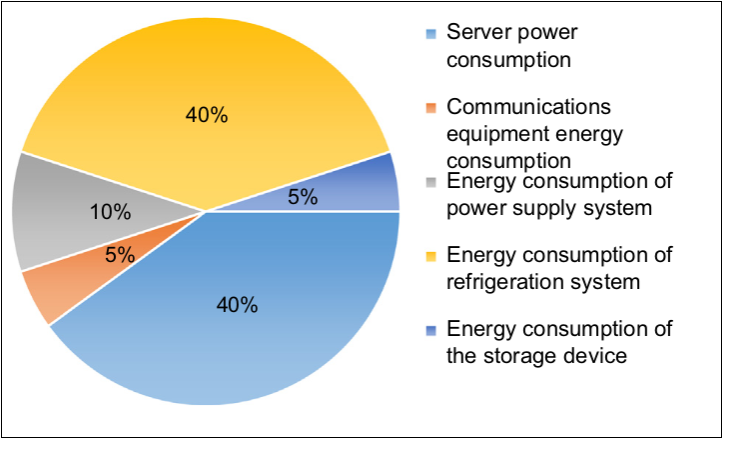
\includegraphics[width=0.5\textwidth]{pics/energyConsumption.png}
	\caption{Energy consumption distribution of data centers \cite{Rong:2016js}}
	\label{fig:consumption}
\end{figure} 

Apart from upfront investment, energy consumption \cite{Kaplan:up01fR-k} is the major expense of data centers. Therefore, it is also the top concern of Cloud providers. Energy consumption is derived from several parts as illustrated in Figure \ref{fig:consumption}. Cooling system and servers or PMs account for a majority of the consumption. A recent survey \cite{Cho:2016kz} shows that the recent development of cooling techniques have reduced its energy consumption and now 
server consumption has become the dominate energy consumption component. 

\begin{figure}
	\centering
	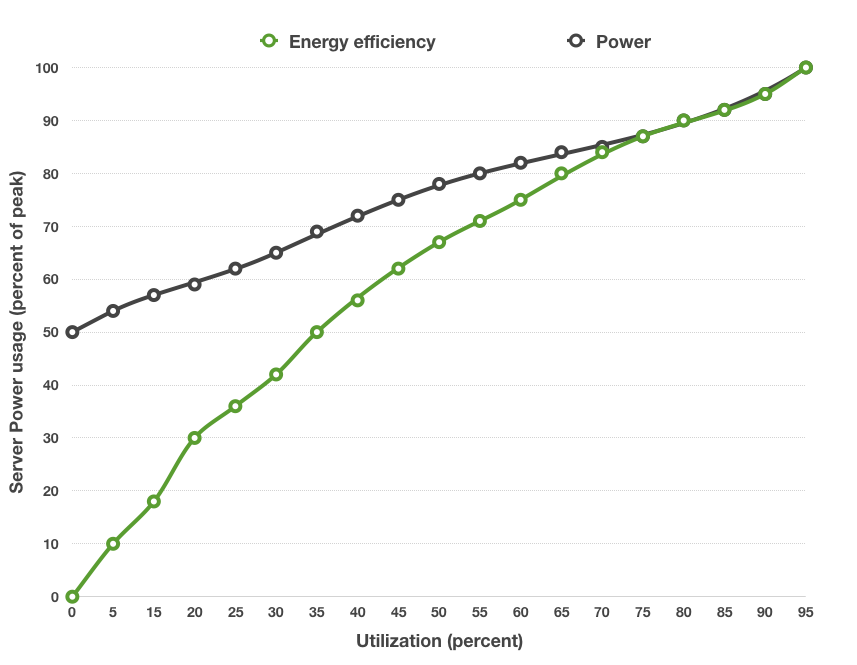
\includegraphics[width=0.5\textwidth]{pics/util.png}
	\caption{Disproportionate between utilization and energy consumption \cite{Barroso:2007jt}}
	\label{fig:unproportional}
\end{figure} 
According to Hameed et al \cite{Hameed:2016cma}, PMs are far from energy-efficient. 
The main reason for the wastage is that the energy consumption of PMs remains high even when the utilization are low (see Figure \ref{fig:unproportional}). Therefore, a concept of \emph{energy proportional computing} \cite{Barroso:2007jt} raised to address the disproportionate between utilization and energy consumption. 


Virtualization \cite{Uhlig:2005do} is the fundamental technology that enables Cloud computing. It partitions a physical machine's resources (e.g. CPU, memory and disk) into several isolated units called virtual machines (VMs) where each VM allows an operating system running on it. This technology rooted back in the 1960s' and was originally invented to enable isolated software testing, because VMs can provide good isolation which means applications running in co-located VMs within the same PM without interfering each other \cite{Somani:2009ho}. Soon, people realized that it can be a way to improve the utilization of hardware resources: With each application deployed in a VM, a PM can run multiple applications. Later, a dynamic migration of VM was invented, which compresses and transfers a VM from one PM to another. This technique allows resource management in real time which inspires the strategy of server consolidation. 


\subsection{Resource Management in IaaS}
The resource management in IaaS can be roughly separated into three \cite{Svard:2015ic, Mishra:2012kx} which are applied in different scenarios: Application initialization, Prediction and Global consolidation, and Dynamic resource management (see Figure \ref{fig:management}). 

\begin{figure}
	\centering
	\begin{subfigure}[b]{0.9\textwidth}
		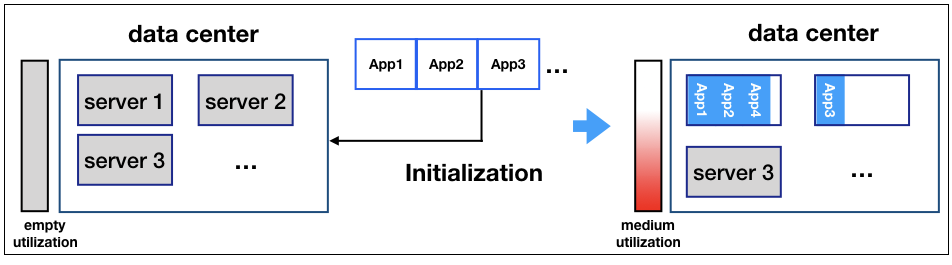
\includegraphics[width=\textwidth]{pics/initialization.png}
		\caption{Initialization}
	\end{subfigure}
	\begin{subfigure}[b]{0.9\textwidth}
		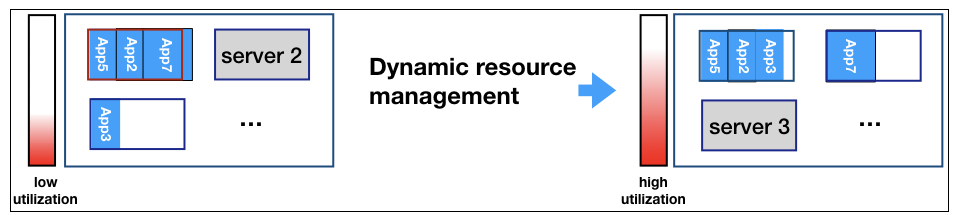
\includegraphics[width=\textwidth]{pics/dynamic_resource.png}
	\caption{Dynamic resource management}
	\end{subfigure}
	\begin{subfigure}[b]{0.9\textwidth}
		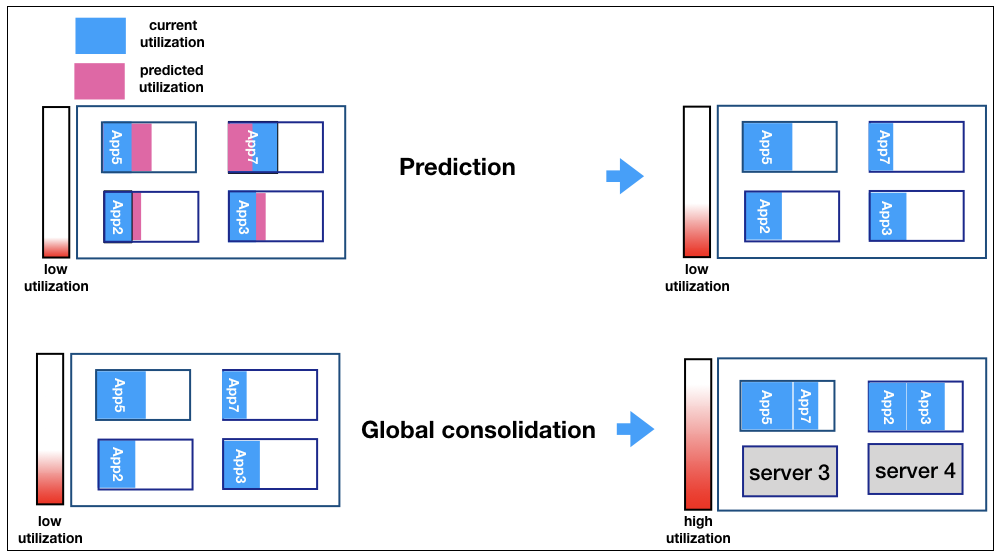
\includegraphics[width=\textwidth]{pics/predict_consolidate.png}
	\caption{Prediction and Consolidation}
	\end{subfigure}
	\caption{Three stages of resource management in IaaS}
	\label{fig:management}
\end{figure}


% Server consolidation is the core functionality involving in all Cloud resource management operations. These operations

% Data center constantly receives new requests for applications initialization. Once the new applications have been allocated, the utilization begins to drop. This is because, initially, applications are compactly allocated on PMs. As old applications instance are released because of canceling, the compact structure become loose. Dynamic resource management is a process which can slow the utilization from decreasing. It consolidates by re-allocating one application at a time. Finally, global consolidation is conducted periodically to dramatically improve the resource utilization.
\begin{enumerate}
	\item \emph{Application initialization} is applied when new applications or new VMs arrive and the problem is to allocate them into a minimum number of PMs.

	In this problem, a set of applications or VMs are waiting in a queue. The resource capacity of the PM and usage by applications are characterized by a vector of resource utilizations including CPU, memory and etc. Then, the allocation system must select a minimum number of PMs to accommodate them so that after the allocation, the resource utilizations remain high. The problem is to consider the different combinations of applications so that the overall resource utilization is high. This problem is naturally modeled as a static bin-packing problem \cite{CoffmanJr:1996ui} which is a NP-hard problem meaning it is unlikely to find an optimal solution of a large problem. 

	\item \emph{Prediction and Global consolidation} is conducted periodically to adjust the current allocation of applications so that the overall utilization is improved.

	In this problem, time is discrete and it can be split into basic time frames, for example: ten seconds. A periodical operation is conducted in every $N$ time frames.
	A cloud data center has a highly dynamic environment with continuous arriving and releasing of applications. Releasing applications cause hollow in PMs; new arrivals cannot change the structure of current allocation. Therefore, after the initial allocation, the overall energy efficiency is likely to drop along with time elapsing. 

	In prediction, an optimization system takes  the current applications' utilization records as the input. Make a prediction of their utilization in the next period of time. 
	In Global consolidation, based on the predict utilization and the current allocation - including a list of applications/VMs and a list of PMs, the system adjusts the allocation so that the global resource utilization is improved.

	In comparison with initialization, instead of new arrivals, the global consolidation considers the previous allocation. Another major difference is that global consolidation needs to minimize the differences of allocation before and after the optimization. This is because the adjustment of allocation relies on a technique called live migration \cite{Clark:2005uda}, and it is a very expensive operation because it occupies the resources in both the host and the target. Therefore, global optimization must be considered as a time-dependent activity which makes the optimization even difficult.

% In comparison with dynamic consolidation, global consolidation takes a set of VMs as input instead of one. Therefore, it is time consuming and often treated as a static problem.
	\item \emph{Dynamic resource management} 
 	Dynamic resource management is applied in three scenarios. \textbf{First},  it is applied when a PM is overloading. In order to prevent the QoS from dropping, an application is migrated to another PM. This is called hot-spot mitigation \cite{Mishra:2012kx}. \textbf{Second}, it is applied when a PM is under-loading. Under-loading is when a PM is in a low utilization state normally defined by a threshold. At this moment, all the applications in the under-loading PM are migrated to other active PMs, so the PM becomes empty and can be turned off. This is called dynamic consolidation. \textbf{Third}, it is applied when a PM having very high level of utilization while others having low. An adjustment is to migrate one or more application from high utilized PMs to low ones. This is called load balancing.

	No matter which scenario it is, a dynamic resource management always involves three steps . 
	\begin{itemize}
		\item \emph{When to migrate?} refers to determine the time point that a PM is overloaded or underloaded. It is often decide by a threshold of utilization.
		\item \emph{Which application to migrate?} refers to determine which application need to be migrated so that it optimize the global energy consumption.
		\item \emph{Where to migrate?} refers to determine which host that an application is migrated to. This step is called dynamic placement which is directly related to the consolidation, therefore, it is decisive in improving energy-efficiency. 
	\end{itemize}

	Among three operations, dynamic placement is a dynamic and on-line problem.
	The term ``dynamic'' means the request comes at an arbitrary time point. An on-line problem is a problem which has on-line input and requires on-line output \cite{Borodin:uQcy_H6C}. It is applied when a control system does not have the complete knowledge of future events.

	There are two difficulties in this operation, firstly, dynamic placement requires a fast decision while the search space is very large (e.g hundreds of thousands of PMs). Secondly, migrate one application at a time is hard to reach a global optimized state.

\end{enumerate}



Finally, a consolidation plan includes four major items:
			\begin{enumerate}
				\item A list of existing PMs after consolidation
				\item A list of new virtual machines created after consolidation
				\item A list of old PMs to be turned off after consolidation
				\item The exact placement of applications and services
			\end{enumerate}

By the nature of Cloud resource management, server consolidation techniques can also be categories into static and dynamic methods \cite{Xiao:2015ik, Verma:2009wi}. Static method is a time consuming process which is often conducted off-line in a periodical fashion; initialization and global consolidation belong to this category. It provides a global optimization to the data center. Dynamic method adjusts PMs in real time. It often allocates one application at a time. Therefore, it can be executed quickly and often provides a local optimization to the data center.


















% They are bonded by the Quality of service and computing resource. Quality of service and the computing resources are the two sides of a coin. 



% Cloud users deploy their software on Clouds. They want to increase the profit by increasing income and decreasing expense. In order to accomplish this goal, they can attract more End suers by improving the functionality of softwares and the non-functionality features by guaranteeing Quality of Service (QoS). To improve the non-functionality features, Cloud users need to reserve enough resources as well as minimizing the resource so that the cost is low.

% service capacity planning is the core process. The capacity planning has two conflicting objectives, on one hand, it must meet End users' QoS requirement by using enough resources.  On the other hand, the cost must be minimized. In pre-Cloud era, the capacity planning determines the upfront investment in infrastructure, therefore, capacity, reliability, and scalability are all need to be carefully considered and balanced. In Cloud environment, the burden of capacity planning is largely released by elastic resource management and the pay-as-you-go policy.

% Cloud users identify a list of critical QoS parameters called Service Level Agreement (SLA) which specifies the non-functional requirements such as throughput, latency, and availability. These QoS parameters are mapped to resources (e.g. CPU, memory, network bandwidth) which can satisfy these requirements. Violation of SLA will lead to penalty and decreasing in number of users. Therefore, in essence, the key to attract more users is an effective resource management system which can rapidly react to the fluctuating resource demand. 

% Beside increase the income, reduce the expense is another way to improve profit. As previous section mentioned, energy consumption is the main source of expense. In energy consumption, server energy consumption is the core that needs to be improved. 

% \subsection{Energy-aware Resource Management}
% \subsection{An Overview of Evolutionary Computation}


% In order to understand Cloud computing, firstly we will illustrate the five essential elements of Cloud computing and their advantages.

% Cloud computing has five essential elements:
% \begin{enumerate}
%  \item On-demand self-service, it means a Cloud user can require computing resources (e.g CPU time, storage, software use) without the interaction with Cloud provider.
%  \item Broad network access, Computing resources are connected and delivered over the network.
%  \item Resource pool, a Cloud provide has a ``pool'' of resources which are normally virtualized servers. In IaaS, it provides predefined sizes of VMs. In PaaS, the resources are `invisible' to Cloud users who have no knowledge or ability to control. 
%  \item Rapid elasticity, from the perspective of Cloud users, computing resources are assigned and released in
% real time. In addition, the resources assign to their software is ``infinite''. Therefore, Cloud users do not need to worried about the scalability of their applications.
%  \item Measured Service provides an accurate measure of the usage of computing resources. It is fundamental to the pay-as-you-go policy.
% \end{enumerate}

% \textcolor{Blue}{What is your purpose to describe the following content?}
% \textcolor{Red}{
% 	I would like to discuss the differences, advantages of disadvantage of the resource management in different service models. Therefore, after illustrate how they are work. The point is to compare the resource management. And then, lead to a new service model. And the advantage of new service model should be obvious. 
% }\\
% Traditional Cloud computing has three service model as illustrated in Figure \ref{}.
% Infrastructure as a Service (IaaS), Platform as a Service (PaaS), and Software as a Service. 
% \subsection{Resource Management}
% Scope of Cloud computing resource management.
% \begin{enumerate}
%  \item Actors
%  \item Management Objectives
%  \item Resource Types
%  \item Enabling Technologies
% \end{enumerate}






